
\newpage
\section{Discussion}
\label{sec:discussion}
While a lot of research has looked at the performance aspects of Docker containers on client side,
we believe the current registry design is inefficient and 
the massive amount of images will push registry become a bottleneck in the whole
container system.
In this work, we have attempted to solve the redundant data issue 
with seamlessly integrating caching and deduplication guided by user access pattern
to showcase the benefits for both the Docker registry service providers as well as the clients.

We believe that our paper will lead to discussion on the following points of interesting:
(1) The need for a compatible deduplication on registry.
Since deduplication is a well-studied area, we believe that the paper will lead to 
hot discussion on how the extant approaches 
adapt to a diversity data format such as compressed file format.
(2) Issues about how to effectively use cache by exploring user access pattern to improve the performance of whole container system,
and where to place cache, for example, at registry side, remote cloud storage side, or Docker client side
to efficiently benefit container performance. 
(3) The role of layer and image.
The redundant data issue stems from container's storage virtualization technique by using
union file systems to pack everything inside different layers used as a plugin OS image.
An open aspect of our work is improving 
the efficiency of current union file systems and container storage virtualization technique.
%the incompatible issue between current deduplication techniques
%and registry with  
%without mitigating overall performance. 
%In this section, we discuss issues and concerns 
%and additional optimizations to help speed up \sysname.

An unexplored issue is that redundant data in Docker client side, which is
greatly different with registry storage 
because registry stores compressed layers
while client end host storage system stores uncompressed layers.
Therefore, the redundant issue in Docker client side with limited local storage space is
 as much worse as registry storage system.
 However, applying current deduplication methods that are usually deployed on backup storage systems
  on
 client side would largely affect the container runtime performance. 
 This is because performing file-level deduplication on the Docker client side
 requires intensive file fingerprint calculations, and file fingerprint lookup, 
 which will slow down container runtime performance.
 Furthermore, we believe our work can help to synchronize deduplication for both
 client side deduplication with registry side deduplication
 to yield desirable win-win solutions.
 
% For future work, we will offload client-side deduplication to server-side, meaning that the 
% Docker client doesn't need to do deduplication because
% it can push all its created images to the registry and the registry eliminates duplicate files for the client. 
% In this case, Docker clients use the registry as a duplicate file washing machine to 
% remove duplicate files in their local file systems without a performance overhead.
%1. File cache and layer buffer management 
%We observed that although half of the users have only one repository with a few layers, there are some users who own many layers. 
%For future work, we will focus on precisely predicting which layers will be accessed by active users and prefetch them in the cache for later accesses.
%We also observed that 
%\paragraph{How many more "layers" can fit in file cache compared with naively storing layers in file cache}
%\paragraph{Can we do client-side deduplication to remove duplicates}
%In the future work, we will focus on how to efficiently manage file cache and layer buffer
%so that we can facilitate more active user requests.
%For example, where to store prefetch layers?
%Our algorithm requires to 
%fetch a certain amount of layers for all connected users to maintain a higher hit ratio.
%If we store prefetched layers into layer buffer,  it requires a big cache to accommodate these layers.
%So during layer prefetching, if the layer buffer is full, 
%we will put the prefetched
%Our algorithm can efficiently improve the cache hit ratio. 
%However, it requires to fetch a certain amount of layers for all connected users.
%And its hit ratio largely depends on duration threshold.
%If we set a higher duration threshold, we can keep more layers in cache 
%but
%\paragraph{Seamlessly integrating backend dedup process with the prefetching algorithm}
%
%In future work, we will analyze the time it takes to fetch a layer from the backend storage system.
%A high latency for prefetching a layer may affect the response time of subsquent incoming \texttt{pull} layer requests.
%We will also analyze the cost-benefit of prefetching a layer.
%Prefetching a layer from cold repositories can serve an immediate pull request. 
%However, this layer will be evicted from the cache after a short period of time because it won't be accessed again by other users. 
%Prefetching is benefitial, but it is associated with the consumption of a lot of resources such as CPU, network bandwidth, and I/Os. 
%Moreover, prefetching a layer into the cache may trigger the eviction of layers from hot repositories.
%We will also quantify the performance gain by using a file cache.
%Although the file cache can increase space efficiency, a hit in the file cache,
%entails subsquent parallel compression operations that may cause considerable latency.

%Our first question is if we prefetch layers from backend dedup storage system,
%there will a latency added to our prefetch requests, 

%\paragraph{Another approach to reduce redudant data in Docker registry: Docker client-side deduplication}
%
%Client-side deduplication affects the container runtime. 
%This is because performing inline file-level deduplication on the Docker client %side
%requires intensive file fingerprint calculations, and file fingerprint lookup, 
%which will slow down container runtime performance.
%For future work, we will offload client-side deduplication to server-side, meaning that the 
%Docker client doesn't need to do deduplication because
%it can push all its created images to the registry and the registry eliminates duplicate files for the client. 
%In this case, Docker clients use the registry as a duplicate file washing machine to 
%remove duplicate files in their local file systems without a performance overhead.


%
%Data deduplication has proven itself as a highly effective technique for
%eliminating data redundancy.
%%
%In spite of being successfully applied to numerous real datasets, deduplication
%bypassed the promising area of Docker images.
%%
%In this paper, we propose to fix this striking omission.
%%
%We analyzed over 1.7 million real-world Docker image layers and identified that
%file-level deduplication can eliminate 96.8\% of the files resulting in
%a capacity-wise deduplication ratio of 6.9$\times$.
%%
%We proceeded with a simulation-based evaluation of the impact of deduplication
%on the Docker registry performance.
%%
%We found that restoring large layers from registry can slow down \texttt{pull}
%performance due to compression overhead. To speed up \sysname, we suggested several
%optimizations.
%%
%%\VT{After Section 4 is ready, we might add here one interesting finding from
%%simulation.}\NZ{addressed}
%%
%Our findings justify and lay way for integrating deduplication in the Docker registry.
%
%\paragraph{Future work}
%%
%In the future, we plan to investigate the effectiveness of sub-file deduplication for
%Docker images and to extend our analysis to more image tags rather than just the \texttt{latest} tag.
%%
%We also plan to proceed with a complete implementation of \sysname.
%


%\paragraph{Further utilize user behavior pattern to accurately predict layer access pattern}
%%\HA{my thoughts}
%%maybe reserve 5\% or 10\% of cache space to cache the top most requested layers of all time. I assume some OS images like Alpine are used as OS of many Docker images as its the choice OS for Docker instead of ubuntu because ubuntu is much larger in size.
%%We observed that there are some active users but do not access layers, instead, they issued a lot \texttt{get}
%%manifest requests. In our cache algorithm, we already identified and ruled out these users from our cache.
%%However, there are users who issues  
%We observed that although half of the users have only one repository with a few layers, there are some users who own many layers. 
%For future work, we will focus on precisely predicting which layers will be accessed by active users and prefetch them in the cache for later accesses.
%We also observed that 
%
%%\paragraph{How many more "layers" can fit in file cache compared with naively storing layers in file cache}
%%\paragraph{Can we do client-side deduplication to remove duplicates}
%\paragraph{Docker client-side deduplication: viability and implications}
%Client-side deduplication affects the container runtime. 
%Because performing inline file-level deduplication on the Docker client side requires intensive file 
%fingerprint calculations and file fingerprint lookup, which will slow down container runtime performance.
%For future work, we will offload client-side deduplication to server-side, meaning that the 
%Docker client doesn't need to do deduplication because
%it can push all its created images to the registry and the registry eliminates duplicate files for the client. 
%In this case, Docker clients use the registry as a washing machine to launder duplicate files in their local file systems without performance overhead.

%\HA{my thoughts:} 
%There are two things,
%First, client-side deduplication: meaning the client assisting registry deduplication. That is, the client only sends the files that the registry does not have, saving bandwidth, less compute cycles at the registry, making it more available for other requests, eventually improving performance. For this, a server or registry would maintain a list of stored files, the client first sends a check request, then only sends the files not stored at the registry.
%
%Second, client-storage deduplication. For its viability, we need to know how big a Docker client can be, and how much can deduplication benefit and affect client/host performance. 
%
%Maybe, a registry deployed as a cache (a pull through cache) can benefit from deduplication, if its serving a large corporation and employees pull lots of different images.
%\HA{end of my thoughts}



%\begin{compactenumerate}
%%
%\item
%%
%As the majority of the pull time is caused by compression, we propose to cache
%hot layers as precompressed tar files in the staging area.
%
%We observe that only a small proportion of images and layers are frequently
%requested and majority of images and layers are \textit{cold}.
%
%Figure~\ref{fig:pull-cnt} shows the total number of pulls from the time an
%image/layer has been stored in Docker Hub until May 30, 2017.
%
%According to our statistics, only 10\% of all images were pulled
%from Docker Hub more than 360 times from the time the image was first pushed to Docker Hub
%until May 30, 2017. Moreover, we found that 90\% of pulls
%went to only 0.25\% of images based on image pull counts.
%%
%This suggests the existence of both cold and hot images and layers.
%
%\VT{Nannan, can we instead compute that 90\% of pulls
%wen to 0.25\% of images?}
%
%
%translates to only 10\% of layers being pulled more than 660 times (at most).
%
%Note that we calculate the layer pull count shown in Figure~\ref{fig:pull-cnt}
%by aggregating the pull count of all images, which refer to this layer.
%
%Note that the image pull counts are crawled from Docker Hub website.
%
%Actual layer pull counts should be less because pulling an image does not
%necessarily pull all its containing layers if some layer have been previously
%downloaded and are already available locally.
%

%\item
%%
%As deduplication provides significant storage savings, \sysname\ can use faster
%but less effective local compression methods than gzip~\cite{lz4}.
%%
%%\VT{cite a few}
%
%\item
%
%Deduplicating when workload is light As shown above, file-level deduplication
%comes with some performance overhead.
%
%The registries often experience fluctuation in load with peaks and
%troughs~\cite{dockerworkload}.
%%
%Thus, file-level deduplication can be triggered
%when the load is low to prevent interference with 
%client \texttt{pull} and \texttt{push} requests.
%%
%%To further improve the performance of \sysname\, we also suggest to use main
%%memory for temporarily storing and processing \textit{small} layers.
%%
%%According to our findings (see~\S\ref{sec:dedup_ratio}), the majority of
%%layers~(87.3\%) are smaller than 50\,MB and hence can be stored and processed
%%in RAM to speed up deduplication. 
%%
%\end{compactenumerate}

%\begin{figure}
	\centering
	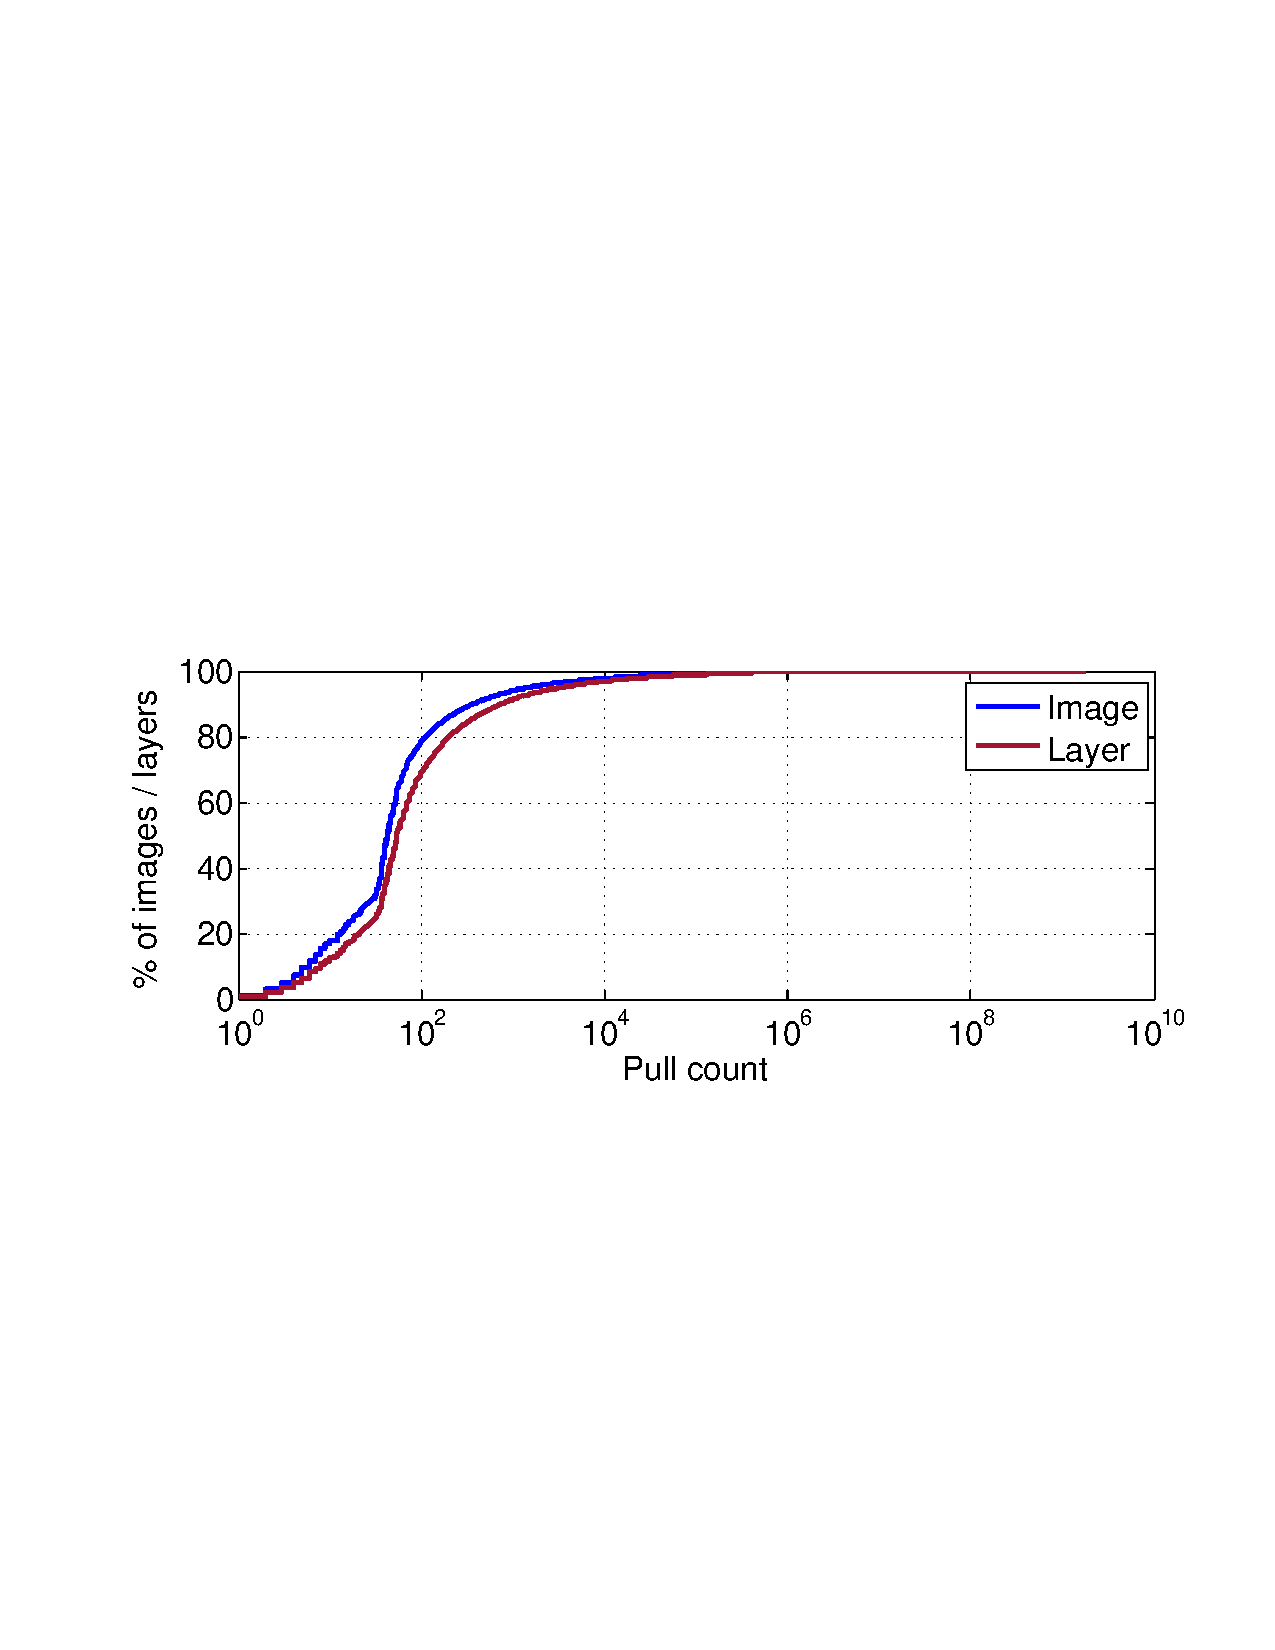
\includegraphics[width=0.4\textwidth]{graphs/pull-cnt.pdf}
	\caption{CDF of layer \& image pull count.
	}
	\label{fig:pull-cnt}
\end{figure}

%=======================================
%|             OLD VERSION              |
%=======================================

%\paragraph{Latency distribution for each operation}
%\subsubsection{When to start file-level dedup?} 

%\paragraph{Latency distribution for each operation}

%\paragraph{Small compression ratio and small layer size}
%
%\begin{figure}[!t]
	\centering
	\subfigure[CDF of compression ratio]{\label{fig_cdf_compression_ratio}
		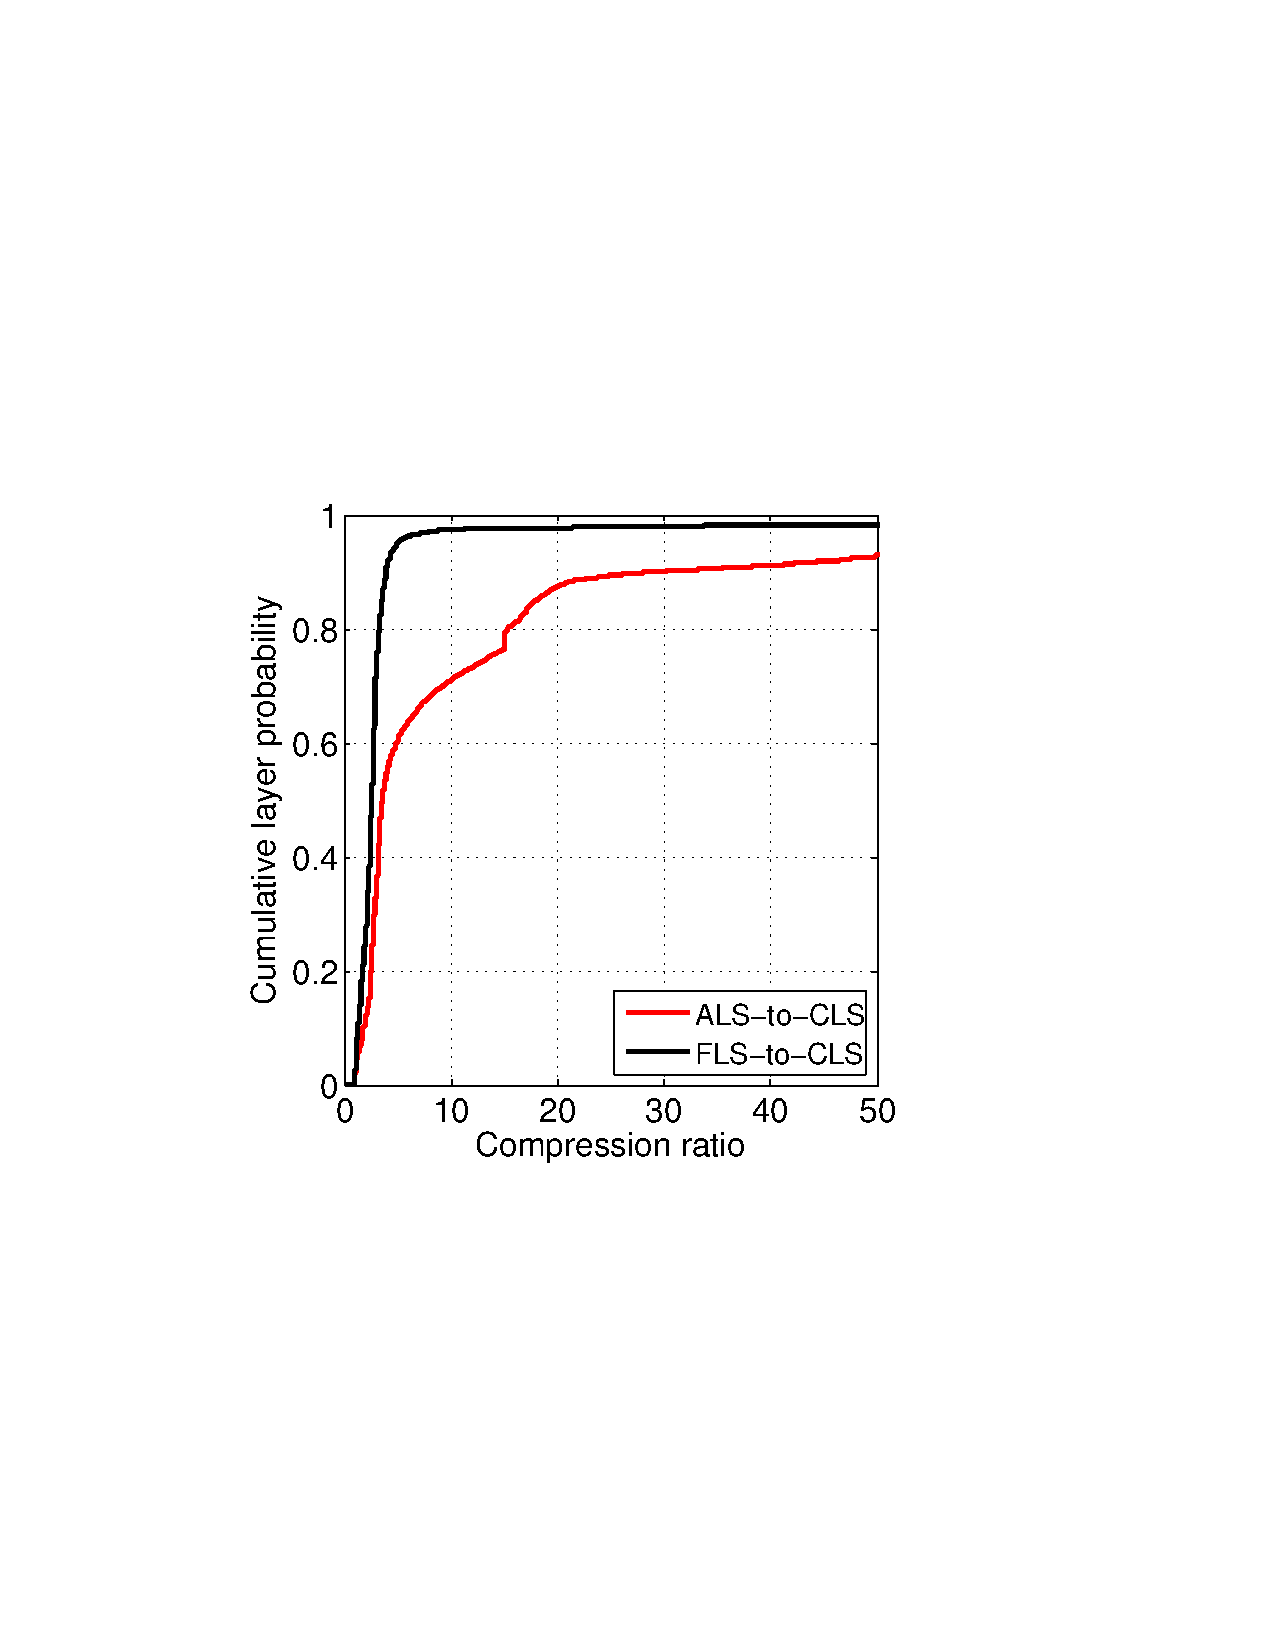
\includegraphics[width=0.23\textwidth]{graphs/cdf_compression_ratio.pdf}
	}
	\subfigure[Histogram of comp. ratios]{\label{fig_his_compression_ratio}
		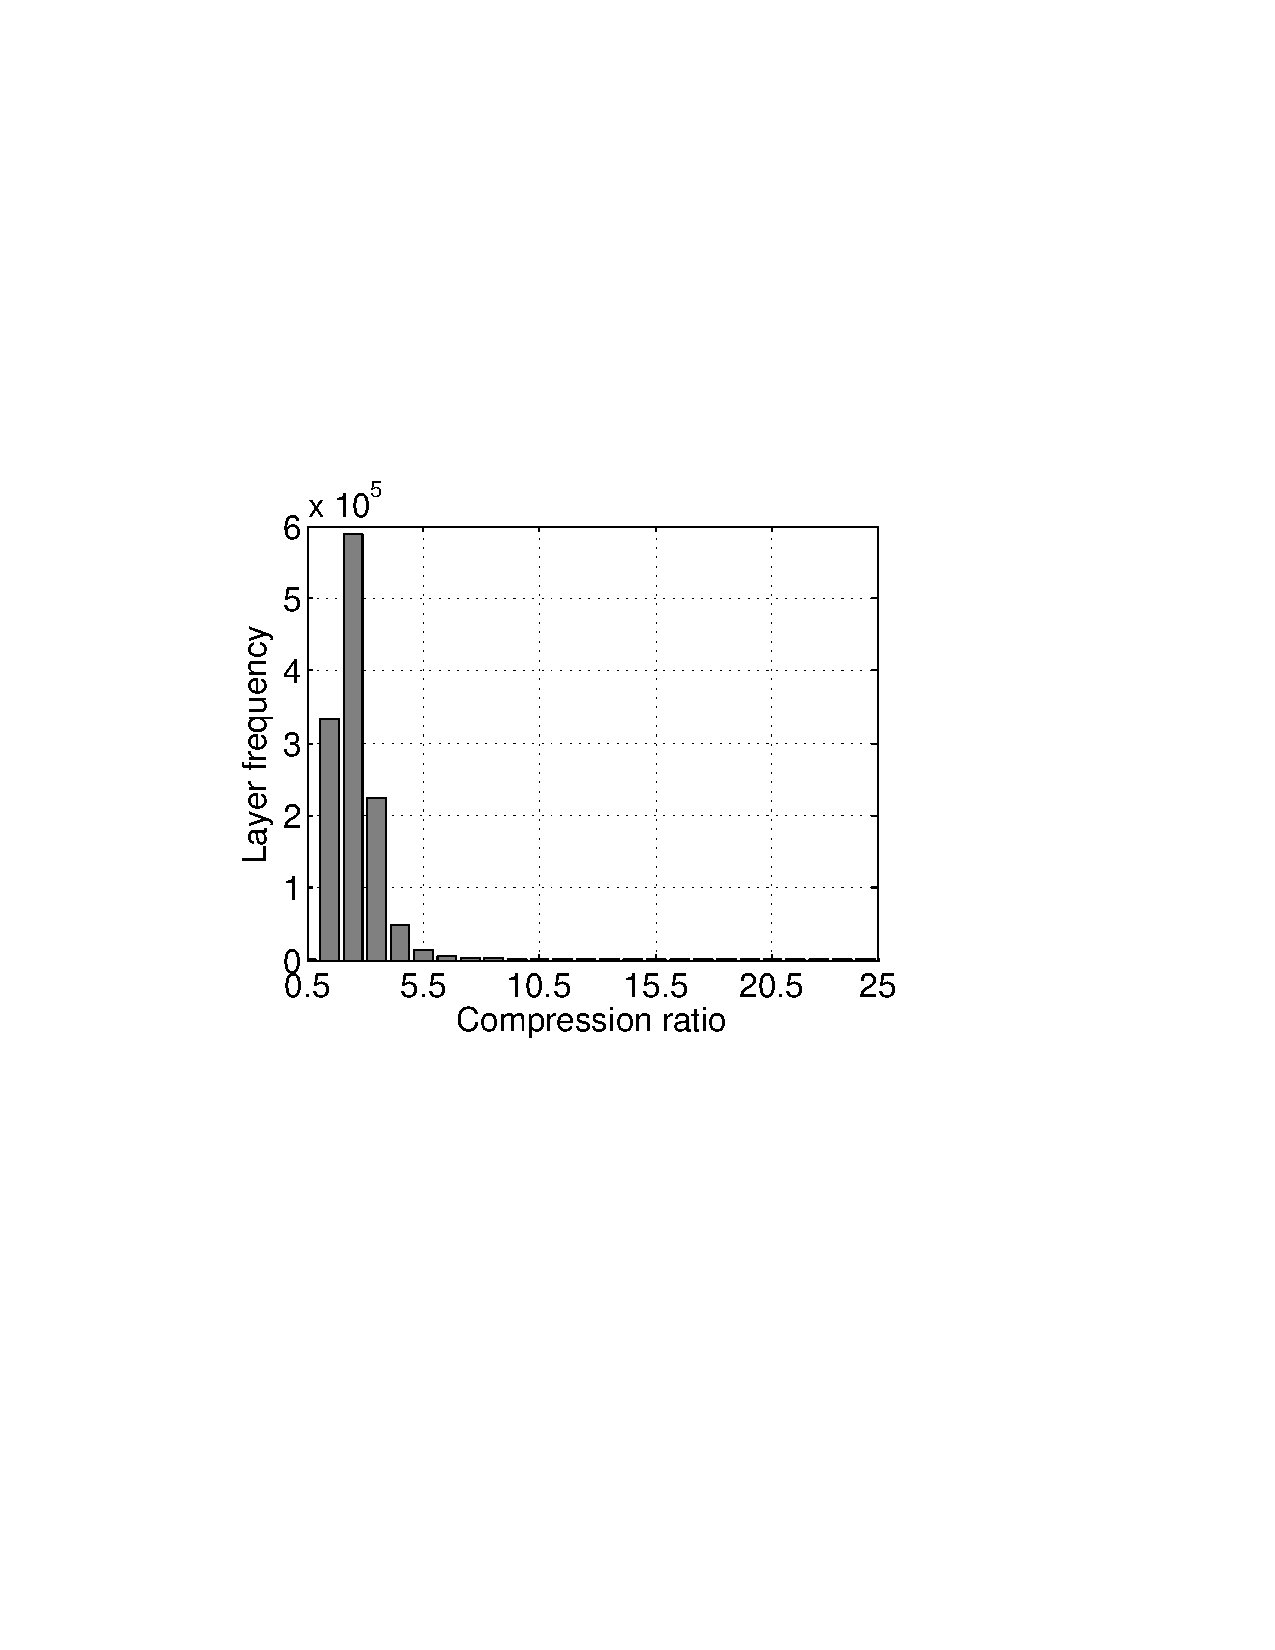
\includegraphics[width=0.223\textwidth]{graphs/his_compression_ratio.pdf}
	}
	\caption{Layer compression ratio distribution
	%\vcomment{Different colors are used in figure (a) and (b) FLS/CLS\nancomment{will address later}}
	}
	\label{fig-compression-ratio}
\end{figure}

%
%\begin{figure}[!t]
	\centering
	\subfigure[CDF of layer sizes]{\label{fig_layer_size_cdf}
		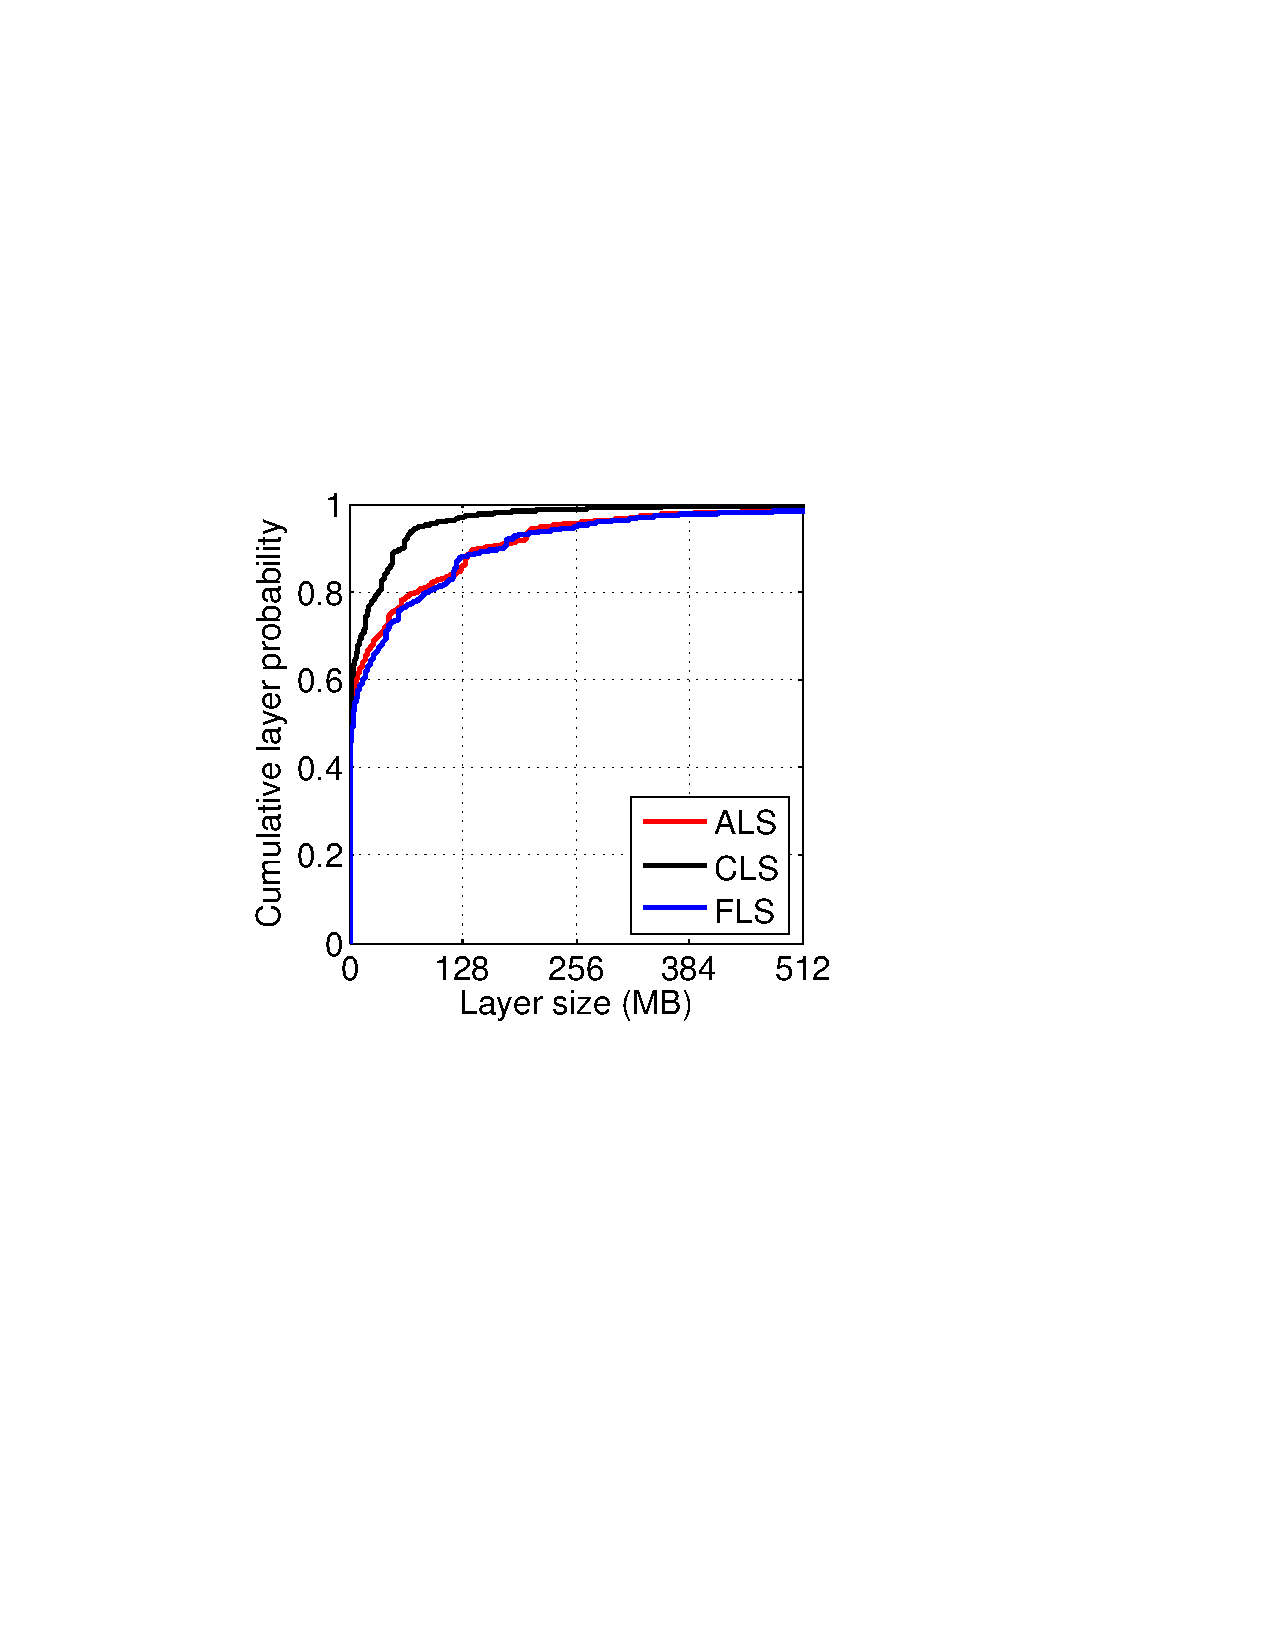
\includegraphics[width=0.234\textwidth]{graphs/layer_size_mb.pdf}
	}
	\subfigure[Histogram of layer sizes]{\label{fig_hist_layer_size}
		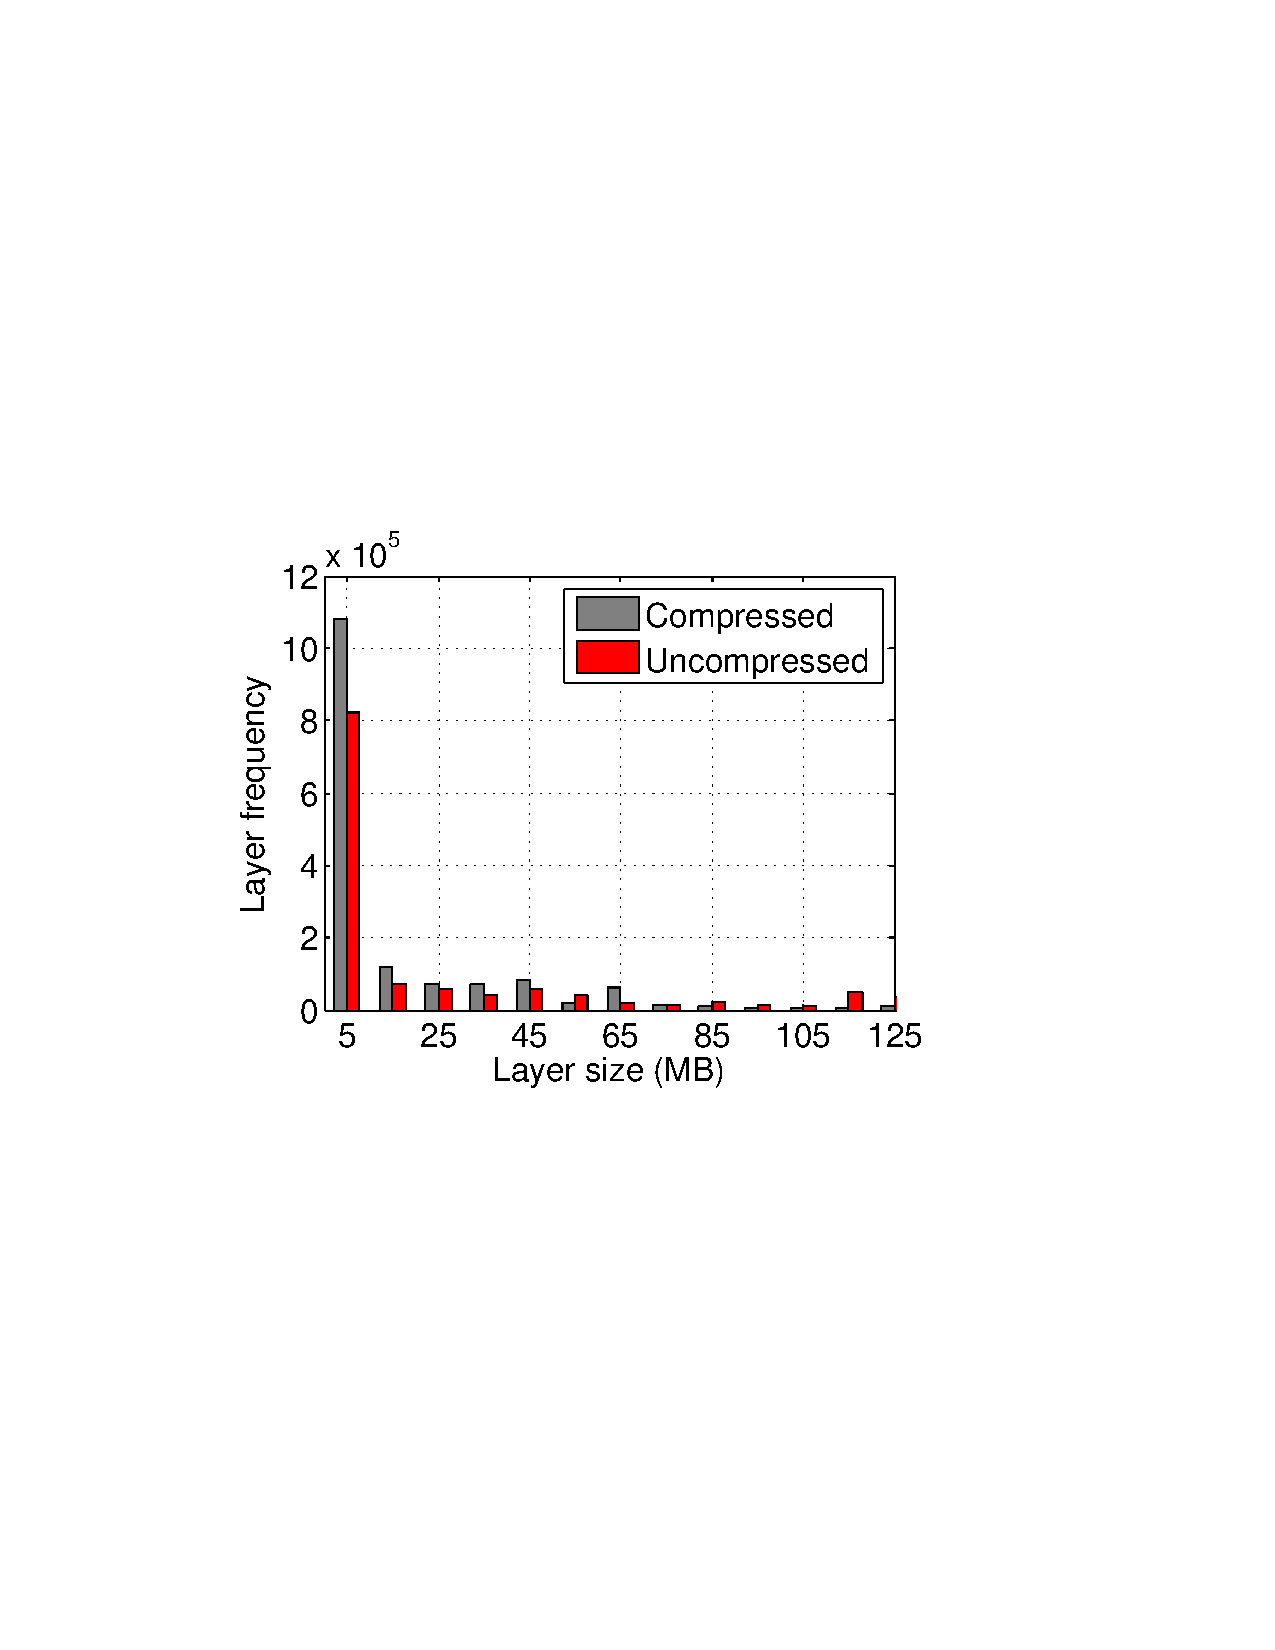
\includegraphics[width=0.213\textwidth]{graphs/hist_layer_size.pdf}
	}
	\caption{Layer size distribution
	\vcomment{Let's use CLS, ALS, and FLS abreviations\nancomment{addressed}}.
	\vcomment{CLS size should go first}.
	\vcomment{We need to use different types of lines (solid, dotted, etc.)
		or markers (round, triangular)}.
	\vcomment{In figure B it is not clear to which bar group corresponds
		  to which layer size. I suggest to try to rotate the graph
		  by 90 grads to fit all layer size labels.\nancomment{aligned label with bar}}
	}
	\label{fig-layer-size}
\end{figure}

%
%We found that most layers'compression ratio is really lower (?) while most of layers have a smaller size. 
%So how about we use archiving instead of compression if the network speed is higher (?GB/s)?

%\paragraph{Network transfer speed is high!}

%\subsubsection{File-level content addressable storage for cold layers}

%\begin{figure}
%	\centering
%	\includegraphics [width=0.45\textwidth]{plots/exp-total-stev-erase.eps}
%	\subfigure[]{\label{fig:per_layer_ratio_fcnt_cdf}
%		\includegraphics [width=0.23\textwidth]{graphs/}
%	}
%	\subfigure[Similar layer dedup]{\label{fig:per_layer_ratio_fcnt_pdf}
%		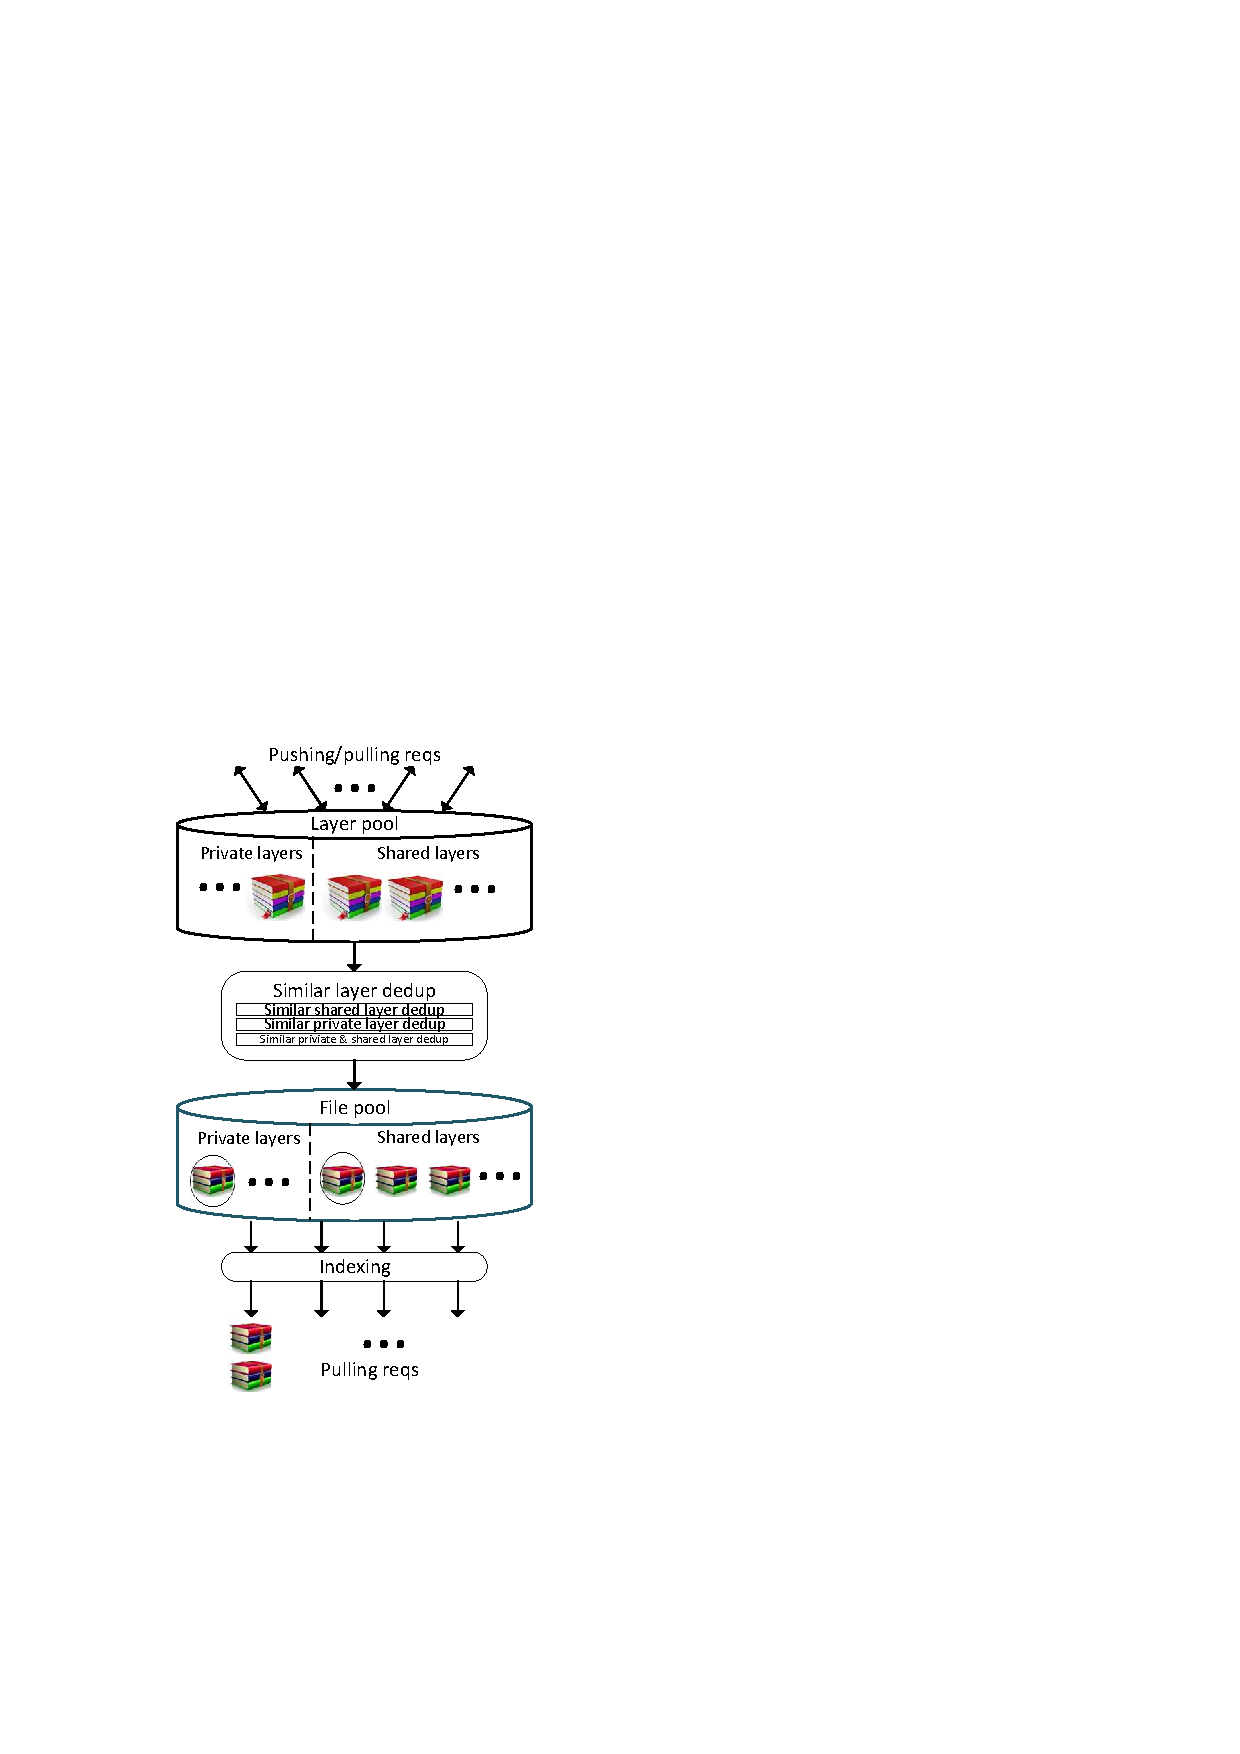
\includegraphics [width=0.22\textwidth]{graphs/graph_reconstruct_layers.pdf}
%	}
%	\caption{File-level content addressable storage model}
%	\label{fig:eval-stdev-erasure-cnt}
%\end{figure}

%\subsection{Hints for performance improvement and storage saving}

%\begin{table} 
%	\centering 
%	\scriptsize  
%	%\begin{minipage}{.5\linewidth}
%	\caption{Latency breakdown} \label{tbl:latency_breakdown} 
%	\begin{tabular}{|l|l|l|l|l|}%p{0.14\textwidth} 
%		\hline 
%		% after \\: \hline or \cline{col1-col2} \cline{col3-col4} ... 
%		% after \\: \hline or \cline{col1-col2} \cline{col3-col4} ... 
%		Operations/latency (S) & max & min & median & avg.\\
%		\hline
%		 gunzip decompression (RAM) & 257.16  & 0.04  & 0.15  & 0.39 \\
% 		\hline
% 		tar extraction (RAM) & 43.41  & 0.04  &  0.14  & 0.18 \\
%		\hline
%		Digest calculation (RAM) & 3455.01  & $<$0.00  & 0.05 & 10.65 \\
%		\hline
%		tar archiving (RAM)  & 53.44 & 0.04 & 0.14 & 0.19\\
%		\hline
%		gzip compression (RAM) & 496.04 & 0.04 & 0.15 & 2.10 \\
%%		\hline
%%		Total time (RAM) (with compression) & & & & \\
%%		\hline
%%		Total time (RAM) (without compression) & & & & \\
%		\hline
% 		\hline
% 		gunzip decompression (SSD) &   &   &    &  \\
% 		\hline
% 		tar extraction (SSD) &   &   &    &  \\
%		\hline
%		Digest calculation (SSD) &  &  & & \\
%		\hline
%		tar archiving (SSD) &  &  & & \\
%		\hline
%		gzip compression (SSD) & &  &  & \\
%%		\hline		 
%%		Total time (SSD) (with compression) & & & & \\
%%		\hline
%%		Total time (SSD) (without compression) & & & & \\
%		\hline
%		\hline
%		Network transfer & 20587.94 & $<$ 0.00 & $<$ 0.00 & 1.20 \\
%		\hline 	
%	\end{tabular} 
%\end{table}


%\begin{table} 
%	\centering 
%	\scriptsize  
%	%\begin{minipage}{.5\linewidth}
%	\caption{Summary of layer \& image characterization} \label{tbl:redundant_ratio} 
%	\begin{tabular}{|l|l|l|l|l|}%p{0.14\textwidth} 
%		\hline 
%		% after \\: \hline or \cline{col1-col2} \cline{col3-col4} ... 
%		% after \\: \hline or \cline{col1-col2} \cline{col3-col4} ... 
%		Metrics & max & min & median & avg.\\
%		\hline
%		Compressed layer size &   &   &   &  \\
%		\hline
%		Uncompressed layer size &   &   &    &  \\
%		\hline
%		Archival size &  &  & & \\
%		\hline
%		Compression ratio &   &   &    &  \\
%		\hline
%		Layer pull cnt. &  &  & & \\
%		\hline
%		File cnt. per layer &  &  & & \\
%		\hline
%		Dir. cnt. per layer &  &  & & \\
%		\hline
%		Layer depth &  &  & & \\
%		\hline
%		\hline
%		Compressed image size &  &  & & \\
%		\hline
%		Uncompressed image size & &  &  & \\
%		\hline
%		Archival image size & &  &  & \\
%		\hline
%		Compression ratio &   &   &    &  \\
%		\hline
%		Image pull cnt.  &  &  & & \\
%		\hline
%		Layer cnt. per image  &  &  & & \\
%		\hline
%		Shared layer cnt. per image  &  &  & & \\
%		\hline
%		File cnt. per layer &  &  & & \\
%		\hline
%		Dir. cnt. per layer &  &  & & \\
%		\hline	
%	\end{tabular} 
%\end{table} 

%\subsection{Constructing shared layers for redundant directories/files}
%
%\paragraph{Smaller number of layers are shared among different images}
%\begin{figure}[!t]
	\centering
	\subfigure[CDF of layer reference count]{\label{fig_repeate_layer}
		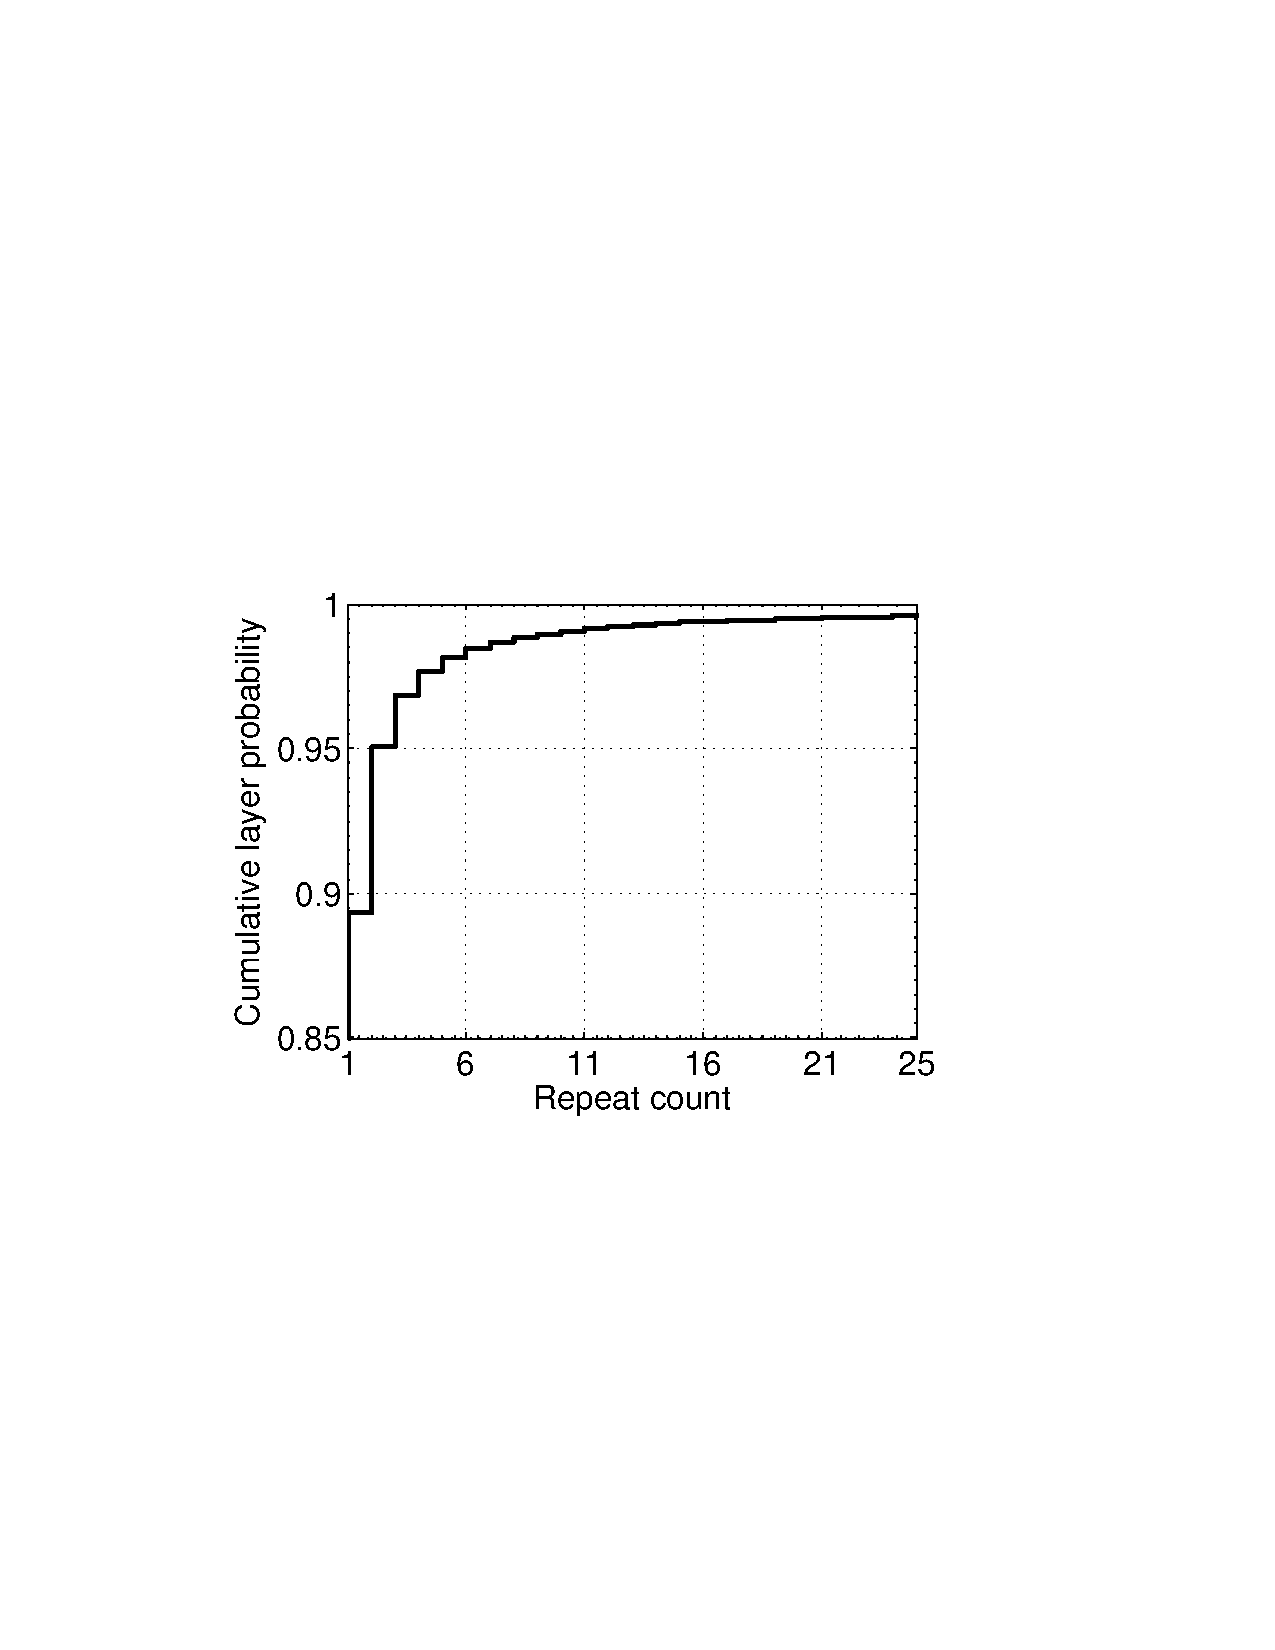
\includegraphics[width=0.23\textwidth]{graphs/repeate_layer.pdf}
	}
	\subfigure[Histogram of layer reference count]{\label{fig_hist_repeate_layer}
		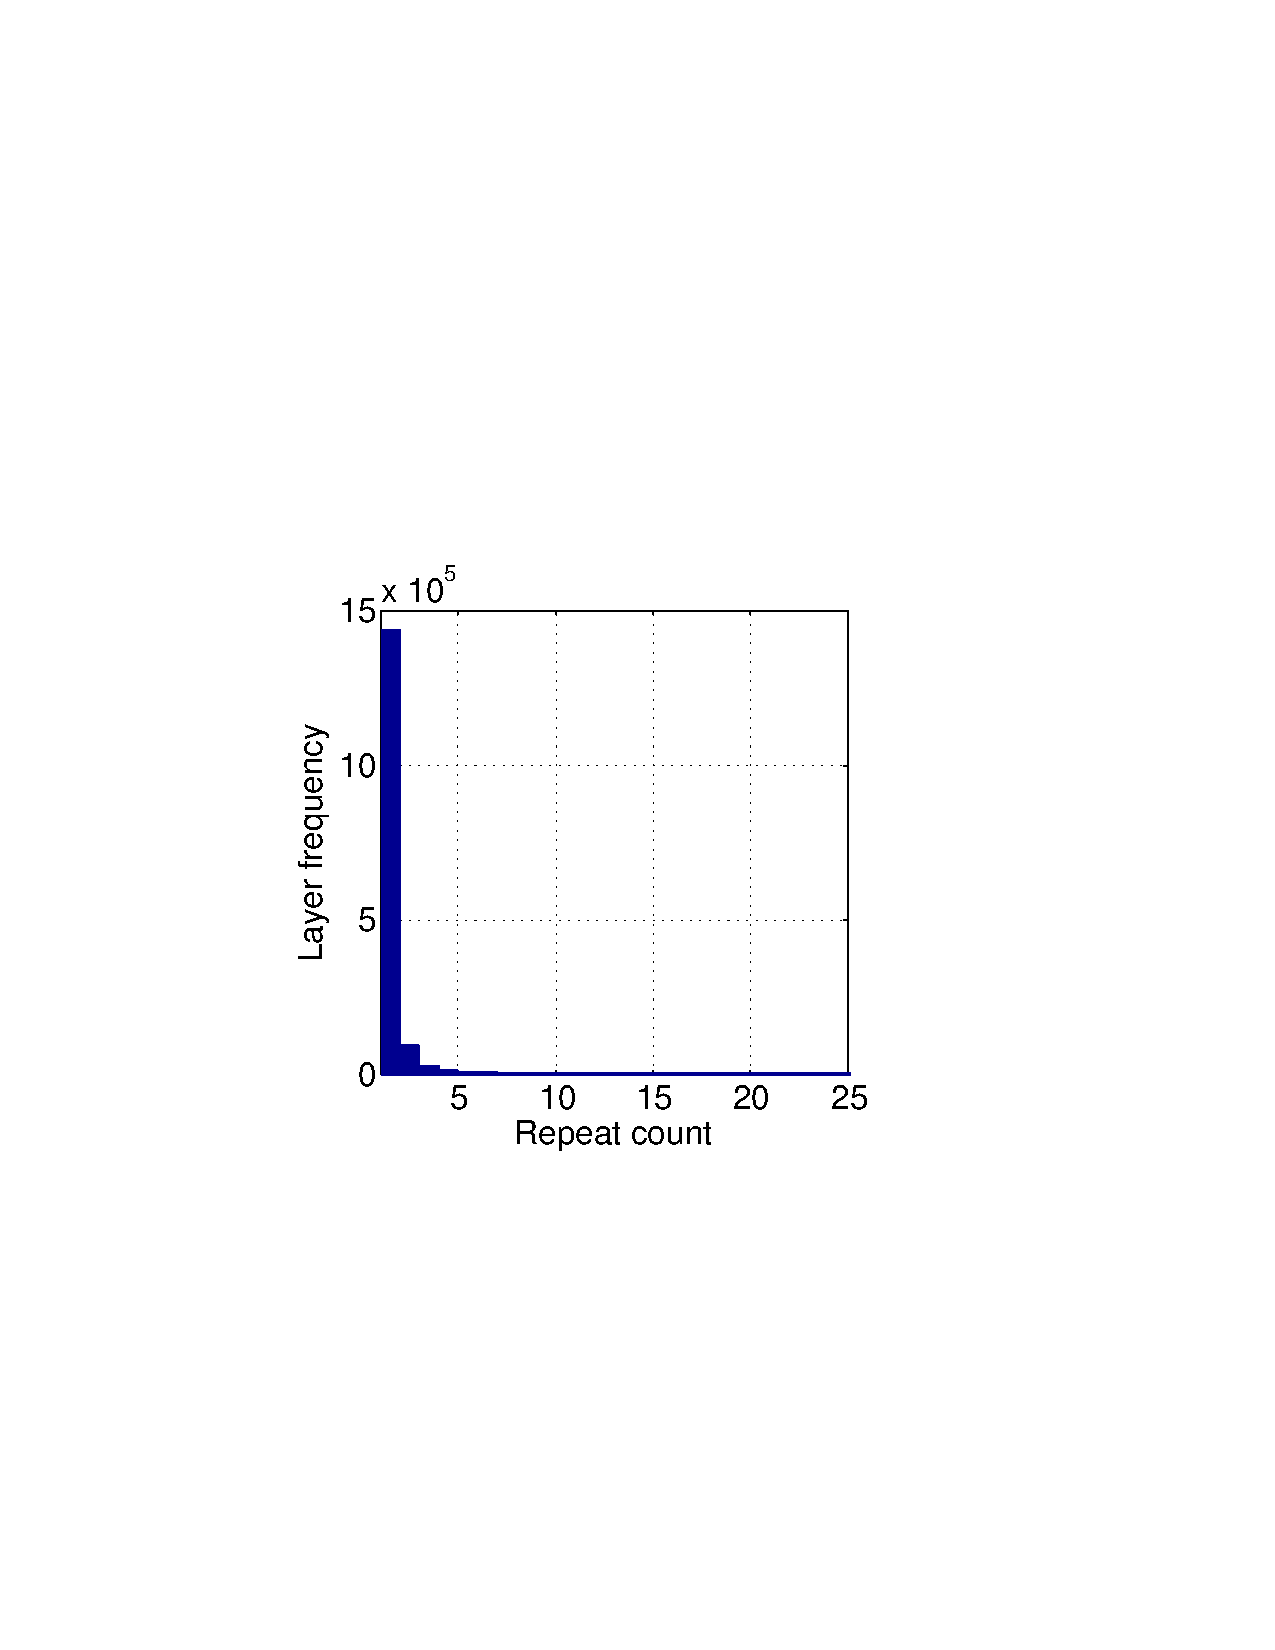
\includegraphics[width=0.223\textwidth]{graphs/hist_repeate_layer.pdf}
	}
	\caption{Layer reference counts across all images}
	\label{fig-repeat-layer-cnt}
\end{figure}
%
%\paragraph{Smaller pull latency than recompression model} the registry can prepare the reconstructed layers before users issue a pull request. But this model requires users to rebuild two layers.

%\subsubsection{Summary of Suggestions/trade-offs between dedup ratio and recompression overhead}
%
%\paragraph{1. using archiving instead of compression}
%\paragraph{2. using file-level dedup for cold images/layers}
%\paragraph{3. using file-level dedup economically}
%When to trigger file-level dedup?
%\paragraph{4. constructing shared layers for redundant dirs/files, for example,}
%%\subsection{Layer reconstruction model}
%%\subsubsection{Reconstruction overhead}
%%\subsubsection{Trade-offs between dedup ratio and reconstruction overhead}
%%\paragraph{Dedup ratio VS. Rebuild overhead}
%%\subsection{Evaluation results}
